\documentclass[journal]{IEEEtran}
\usepackage[T1]{fontenc}
\usepackage[utf8]{inputenc}
\usepackage{amsmath,amssymb,amsfonts}
\usepackage{graphicx}
\usepackage{booktabs}
\usepackage{multirow}
\usepackage{xcolor}
\usepackage{url}
\usepackage{cite}
\usepackage{xspace}
\usepackage{microtype}
\usepackage{balance}

% Cross-references to the main paper: frozen label numbers generated by
% make_supplement_refs.py (see that script). This replaces the xr package,
% which cannot work on Overleaf because main.aux is never visible from the
% supplement's compile sandbox.
\makeatletter
% main-refs.tex -- label numbers of the MAIN paper, frozen for the
% supplement's cross-references.
%
% GENERATED by make_supplement_refs.py from main.aux -- do not edit by hand.
% Regenerate whenever the main paper's numbering changes:
%   pdflatex main.tex && python make_supplement_refs.py
\newlabel{eq:cell_average}{{1}{3}}
\newlabel{eq:correction_system}{{15}{4}}
\newlabel{eq:forward_operator}{{4}{3}}
\newlabel{eq:recovery_fraction}{{24}{8}}
\newlabel{eq:weighted_variational}{{17}{4}}
\newlabel{eq:zero_correction_bound}{{18}{4}}
\newlabel{sec:controlled_synthetic}{{\mbox  {IV-B}}{5}}
\newlabel{sec:exp_config}{{\mbox  {IV-E}}{7}}
\newlabel{sec:generalization}{{\mbox  {VI-D}}{12}}
\newlabel{sec:hpx_datacube_implications}{{\mbox  {VI-F}}{13}}
\newlabel{sec:psf_mismatch}{{\mbox  {IV-E}1}{7}}
\newlabel{sec:real_downscale_experiment}{{\mbox  {IV-D}}{5}}
\newlabel{sec:real_downscale_multiregion_results}{{\mbox  {V-F}}{9}}
\newlabel{sec:rl_ablation}{{\mbox  {V-C}}{9}}
\newlabel{sec:roundtrip_interpretation}{{\mbox  {VI-A}0a}{11}}
\newlabel{sec:synthetic_results}{{\mbox  {V-A}}{8}}

\makeatother
\graphicspath{{figures/}}

\newcommand{\healpix}{HEALPix\xspace}
\newcommand{\dggs}{DGGS\xspace}
\newcommand{\utm}{UTM\xspace}
\newcommand{\psf}{PSF\xspace}
\newcommand{\R}{\mathbb{R}\,}
\newcommand{\Nside}{N_{\mathrm{side}}\,}
\newcommand{\argmin}{\mathop{\mathrm{arg\,min}}\,}

\renewcommand{\thesection}{S\arabic{section}}
\renewcommand{\thesubsection}{\thesection.\Alph{subsection}}
\renewcommand{\thesubsubsection}{\thesubsection.\arabic{subsubsection}}
\renewcommand{\thefigure}{S\arabic{figure}}
\renewcommand{\thetable}{S\Roman{table}}
\renewcommand{\theequation}{S\arabic{equation}}

\begin{document}

\title{Supplementary Material for ``\texttt{healpix-resample}: PSF-Aware Resampling of Earth-Observation Imagery onto HEALPix''}

\author{
Jean-Marc Delouis\textsuperscript{1},
Tina Odaka\textsuperscript{2},
Benoit Bovy\textsuperscript{3},
Etienne Cap\textsuperscript{4},
Thomas Davison\textsuperscript{5},
Anne Fouilloux\textsuperscript{6},
Camille Gueguen\textsuperscript{7},
Alexander Kmoch\textsuperscript{8},
Justus Magin\textsuperscript{9},
Pablo Richard\textsuperscript{10},
and Vincent Dumoulin\textsuperscript{11}%
\thanks{\textsuperscript{1}LOPS UMR 6523,
CNRS--IFREMER--IRD--Univ. Brest--IUEM, Plouzané, France.
Corresponding author: jean.marc.delouis@ifremer.fr. ORCID: 0000-0002-0713-1658.}%
\thanks{\textsuperscript{2}LOPS UMR 6523,
CNRS--IFREMER--IRD--Univ. Brest--IUEM, Plouzané, France.
Email: Tina.Odaka@ifremer.fr. ORCID: 0000-0002-1500-0156.}%
\thanks{\textsuperscript{3}GEORODE, Liège, Belgium.
Email: bbovy@georode.com. ORCID: 0009-0001-4011-3574.}%
\thanks{\textsuperscript{4}LOPS UMR 6523,
CNRS--IFREMER--IRD--Univ. Brest--IUEM, Plouzané, France.
Email: Etienne.Cap@ifremer.fr. ORCID: 0009-0007-0360-0692.}%
\thanks{\textsuperscript{5}European Space Agency (ESA)---ESRIN, Frascati, Italy.
Email: Thomas.Davison@esa.int. ORCID: 0000-0002-0917-4256.}%
\thanks{\textsuperscript{6}LifeWatch ERIC, Seville, Spain.
Email: anne.fouilloux@lifewatch.eu. ORCID: 0000-0002-1784-2920.}%
\thanks{\textsuperscript{7}LOPS UMR 6523,
CNRS--IFREMER--IRD--Univ. Brest--IUEM, Plouzané, France.
Email: camille.gueguen@ifremer.fr. ORCID: 0009-0008-3748-9395.}%
\thanks{\textsuperscript{8}University of Tartu,
Institute of Ecology and Earth Sciences,
Landscape Geoinformatics Lab, Tartu, Estonia.
Email: alexander.kmoch@ut.ee. ORCID: 0000-0003-4386-4450.}%
\thanks{\textsuperscript{9}LOPS UMR 6523,
CNRS--IFREMER--IRD--Univ. Brest--IUEM, Plouzané, France.
Email: Justus.Magin@ifremer.fr. ORCID: 0000-0002-4254-8002.}%
\thanks{\textsuperscript{10}Pablo Richard EI, Paris, France.
Email: pablorichard@hotmail.fr. ORCID: 0000-0002-5441-8213.}%
\thanks{\textsuperscript{11}European Space Agency (ESA)---ESRIN, Frascati, Italy.
Email: vincent.dumoulin@esa.int. ORCID: 0000-0001-5049-3817.}%
}

\markboth{Supplementary Material}{Delouis \MakeLowercase{\textit{et al.}}: Supplementary Material}
\maketitle

\begin{abstract}
This supplement provides the complete illustrative-scene tables and spectral
diagnostics, acquisition and baseline details, hold-out and round-trip
controls, noise and geolocation sweeps, throughput scaling, and the derivation
and ERA5 evaluation of two optional conservative resamplers.
\end{abstract}

\section{Detailed Validation Protocol}
\label{supp:protocol}

\subsection{Controlled Synthetic Detector}

For each of the four illustrative scene classes, Esri World Imagery is used
as a high-resolution spatial texture rather than as a Sentinel-2 radiometric
reference \cite{esri_world_imagery}, read from the pinned Wayback release
26334 (2026-08-05) so that the texture inputs are versioned and
reproducible. Imagery is sampled at Web Mercator zoom
17, converted to grayscale luminance, and evaluated on a grid oversampled by
a factor four relative to the 10~m detector grid. The texture is convolved
with an isotropic Gaussian using reflective boundary conditions and then
averaged over $4\times4$ blocks. The block average is a 10~m square aperture
that the scalar Gaussian inverse does not model. The nominal Gaussian has
$\sigma_G=5.31$~m, the aperture has per-axis
$\sigma_{\mathrm{box}}=10/\sqrt{12}=2.89$~m, and the combined second moment
corresponds to an equivalent Gaussian FWHM of 14.23~m, 13.9\% above the
nominal 12.5~m. The exact kernel remains a Gaussian convolved with a square,
so the experiment is Gaussian-width-matched rather than exactly
response-matched. No additional noise is added in the principal comparison;
Section~\ref{sec:noise_matched} tests noise explicitly.

The nominal Gaussian scale is $s_{\mathrm{op}}=s_{\mathrm{gen}}=10.62$~m,
corresponding to FWHM 12.5~m. The target is nested level-20 \healpix, with
$N_{\mathrm{side}}=2^{20}$ and equivalent cell size 6.22~m. Each source
sample is linked to the nearest cells required to retain at least 99\% of the
kernel weight: $q=22$ for the nominal arm, 48 for the $+50\%$ arm, and 9 for
the $-50\%$ arm. Cells with accumulated influence below 0.1 are excluded.
All three arms use $\lambda=10^{-3}$, at most 14 weighted-CG iterations, and
relative residual tolerance $10^{-8}$.

The high-resolution reference at level 20 is approximated by sampling the
texture at the centres of the 16 nested level-22 children of each retained
level-20 cell and averaging them. The same child-average procedure is applied
to every raster baseline, so all methods target the same footprint-average
estimand. Spectra are computed after independent 1st--99th percentile
normalization, clipping to $[0,1]$, mean subtraction, a two-dimensional Hann
window, and azimuthal averaging of squared Fourier amplitudes.

\subsection{Comparator Configuration}

Nearest-neighbor, bilinear, and bicubic interpolation are evaluated on the
same retained cells and child-average readout. Richardson--Lucy uses
\texttt{skimage.restoration.richardson\_lucy} version 0.26.0: source data are
rescaled to $[0,1]$, deconvolved for 100 fixed iterations with
\texttt{clip=False}, returned to the original radiometric scale, bicubically
upsampled to an intermediate 5~m grid, and averaged over level-22 children.
The Gaussian is converted to source-pixel sigma and truncated at $4\sigma$.
The Fourier Tikhonov baseline uses
$\widehat x=H^*y/(|H|^2+\lambda_{\mathrm{Tik}})$ with
$\lambda_{\mathrm{Tik}}=10^{-2}$ and circular FFT boundaries. These are
fixed configurations; neither setting was selected on held-out calibration
regions.

A definitive tuned comparison should split regions before inspecting method
scores, use one global calibration subset shared by all methods, and select a
single parameter per method by mean region-level RMSE: for example,
Richardson--Lucy iteration count, $\lambda_{\mathrm{Tik}}$, and the proposed
method's damping over predeclared grids. The selected values must then be
frozen and evaluated on disjoint regions, without per-scene or per-region
tuning. The tables below do not claim that protocol has been executed; they
report only the stated fixed configurations.

\subsection{Zero-Correction Reference Ablation}
\label{supp:xref_ablation}

The normalized aggregate $\mathbf x_{\mathrm{ref}}=\mathbf B\mathbf y$ is the
zero-correction arm of the proposed estimator. Equation~\eqref{eq:zero_correction_bound}
of the main paper guarantees that the solved correction cannot increase the
regularized weighted observation-space objective relative to this arm. That
guarantee is not a statement about RMSE to the latent cell-average reference.
A numerical image-domain ablation must therefore export
$\mathbf x_{\mathrm{ref}}$ from the same resampler instance, align its
\texttt{cell\_ids} with the latent reference, and compute the same interior-cell
RMSE, recovery fraction, and paired region statistics as for the full
solution.

In the released implementation this field is computed immediately before CG
as \texttt{x\_ref = y\_filled @ self.M}. The ablation extracts it through
the estimator's own public interface by solving with \texttt{max\_iter=0}:
the CG loop body never executes, the correction stays at its zero initial
vector, and the returned field is exactly
$\mathbf x_{\mathrm{ref}} + \mathbf 0$, with identical operator
construction, NaN handling, support threshold, and cell ids as the full
solve. Nothing is reimplemented, so the two arms cannot diverge.

Executed over the 40 regions of the reduced-resolution validation, the
aggregate alone is the weakest method tested: mean RMSE $0.0180$
(agriculture), $0.0164$ (forest), $0.0381$ (urban), and $0.0029$ (water),
above nearest-neighbor interpolation in every class. The full solution
improves on it in all 40 regions (exact two-sided sign test
$p=1.8\times10^{-12}$; paired difference $0.0061$ [$0.0044$, $0.0080$]),
with mean relative gains of $21.6$--$33.5\%$ by class and per-region gains
of $8.8$--$50.3\%$. The main paper reports this result in its
reduced-resolution results section.

\subsection{Geographically Distributed Synthetic Sample}

Ten regions per scene class are selected as a stratified, geographically
distributed sample, not as a random planetary sample. Each region supplies a
deterministic $3\times3$ lattice of non-overlapping $256\times256$ patches
with 4~km spacing. The independent statistical unit is the region; the nine
patches are spatially correlated subsamples. Two of the 90 selected water
patches lie on homogeneous Caspian Sea water for which the imposed blur has
numerically zero RMSE, making the recovery fraction undefined. This
pre-reconstruction criterion leaves 358 analyzed patches.

Region-cluster confidence intervals use 5000 bootstrap replicates, resampling
regions with replacement and averaging their patches. They describe
variation among the selected regions, not global class uncertainty. The
recovery fraction is Eq.~\eqref{eq:recovery_fraction} of the main paper;
paired differences always compare methods on the same patch or region.

\subsection{Controlled Reduced-Resolution Protocol and Acquisition Screens}

The real-data protocol starts from a native 10~m Sentinel-2 Level-2A B04
patch. The primary level-19 reference is constructed before the tested
degradation: the undegraded image is transferred to level 20 with the nominal
12.5~m operator and its children are geometrically averaged to level 19. In a
separate path, the native image is blurred to 25~m FWHM and point-sampled
every other pixel to form a 20~m observation. Decimation is used instead of a
$2\times2$ average to avoid an additional boxcar component. The observation
is reconstructed to the same level-19 support with an assumed 25~m response;
evaluation excludes cells within 200~m of the boundary. The anisotropic
control uses a 24~m by 45~m degradation but retains the isotropic 25~m inverse
and a 360~m edge margin.

The protocol is repeated at the same 40 anchors as the synthetic experiment.
Real acquisitions are obtained primarily from the Element~84 Earth Search
catalogue \cite{earthsearch}; four European patches are read from the EOPF
Zarr demonstration service. Products are selected deterministically by
lowest cloud cover. Pre-reconstruction screens reject clipped windows,
no-data holes, flat patches, cloud or snow despite low granule-level cloud
fraction, and regions with less than half the median interior-cell count. All
40 regions pass. Reprojection of each reference-cell centroid into the local
UTM frame gives a maximum 6.3~m displacement from the intended patch centre.

A second reference removes shared estimator machinery: native pixels are
assigned to level-19 cells and averaged without a response model or inversion.
The response-width sweep holds the degradation at 25~m while using assumed
inverse widths $\{0.5,0.8,1.0,1.2,1.5\}\times25$~m and a common evaluation
margin. The random-pixel hold-out removes 10\% of source pixels before
operator construction and predicts them from the field fitted to the
remaining 90\%; it is an interpolation test, not a blocked geographic test.

\section{Illustrative Synthetic Results}
\label{supp:synthetic_results}

Table~\ref{tab:synthetic_metrics} reports the RMSE of each
reconstruction relative to both the pre-degradation Esri texture and
the corresponding \psf-blurred observation. The matched
\psf-aware reconstruction is the closest to the pre-degradation
reference for all four scene types. Its RMSE is lower than the
degradation introduced by the prescribed blur by approximately
$17$--$22\%$, showing a modest but systematic partial recovery
of spatial information.

The geometric baselines remain closer to the blurred observation:
they interpolate already degraded samples, so their low RMSE
against the blurred reference reflects preservation of the input
blur rather than recovery of the latent texture.

Errors in the assumed response width act asymmetrically. The
$-50\%$ arm under-corrects and remains under-restored in every
scene. The $+50\%$ arm compensates for more attenuation than is
present and amplifies weakly constrained high-frequency components,
making it consistently the more damaging of the two: its aggregate
RMSE exceeds both the matched result and the original degradation.
The common damping limits but does not remove this amplification,
which the spectral diagnostics of
Section~\ref{sec:spectral_behaviour} show directly.
One caveat applies to the $-50\%$ arm specifically: its kernel is
narrow relative to the target lattice ($\sigma\approx0.43$
level-20 cell widths, $q=9$ support), a regime in which the discrete
cell lattice no longer samples the Gaussian cleanly and the
delivered response acquires a phase-dependent effective width and a
mild anisotropy even for an isotropic specification, so part of the
$-50\%$ behaviour may reflect lattice sampling of the narrow kernel
rather than width error alone; the $+50\%$ conclusions are
unaffected.

Under the fixed configurations reported here, Richardson--Lucy uses the
nominal generation Gaussian but deconvolves on the \utm grid before a
separate cell-average transfer to \healpix; it has higher RMSE than the
proposed configuration in all four illustrative scenes. The same ordering is
observed for the fixed Tikhonov configuration. Matching the estimand removes
one source of unfairness, but these results neither isolate the sequential
structure as the cause of the gap nor establish a ranking against globally
tuned pipelines.

\begin{table*}[t]
\centering
\caption{RMSE in the controlled synthetic-detector experiment over
the common \healpix cells. The matched and both width-mismatch
configurations use $\lambda=10^{-3}$; $+50\%$ and $-50\%$ denote
overestimated and underestimated operator widths. \emph{Estimated
vs.\ no-\psf} measures recovery of the pre-degradation Esri texture,
whereas \emph{Estimated vs.\ \psf} measures closeness to the blurred
observation. Richardson--Lucy uses the matched PSF followed by
bicubic upsampling and cell-average regridding. Lower is better;
bold marks the minimum in each row. Low geometric-baseline errors
against \emph{Esri PSF} reflect preservation of the input blur, not
restoration quality.}
\label{tab:synthetic_metrics}
\setlength{\tabcolsep}{4pt}
\begin{tabular}{llrrrrrrr}
\toprule
 &  & PSF-aware & PSF-aware & PSF-aware & Richardson--Lucy & Nearest & Bilinear & Bicubic \\
 &  &  & $+50\%$ & $-50\%$ & &  &  &  \\
Scene & Comparison &  &  &  &  &  &  &  \\
\midrule
\multirow[t]{3}{*}{urban} & Estimated vs. Esri pre-degradation & \textbf{0.0684} & 0.1427 & 0.0980 & 0.0823 & 0.1057 & 0.1051 & 0.0960 \\
 & Estimated vs. Esri PSF & 0.0525 & 0.1802 & 0.0311 & 0.0189 & 0.0420 & 0.0244 & \textbf{0.0135} \\
 & Esri PSF vs. Esri pre-degradation (degradation) & 0.0859 & - & - & - & - & - & - \\
\cline{1-9}
\multirow[t]{3}{*}{water} & Estimated vs. Esri pre-degradation & \textbf{0.0211} & 0.0456 & 0.0313 & 0.0256 & 0.0343 & 0.0338 & 0.0305 \\
 & Estimated vs. Esri PSF & 0.0170 & 0.0590 & 0.0102 & 0.0066 & 0.0148 & 0.0083 & \textbf{0.0044} \\
 & Esri PSF vs. Esri pre-degradation (degradation) & 0.0274 & - & - & - & - & - & - \\
\cline{1-9}
\multirow[t]{3}{*}{forest} & Estimated vs. Esri pre-degradation & \textbf{0.0242} & 0.0464 & 0.0334 & 0.0284 & 0.0364 & 0.0355 & 0.0326 \\
 & Estimated vs. Esri PSF & 0.0171 & 0.0572 & 0.0105 & 0.0064 & 0.0154 & 0.0080 & \textbf{0.0044} \\
 & Esri PSF vs. Esri pre-degradation (degradation) & 0.0295 & - & - & - & - & - & - \\
\cline{1-9}
\multirow[t]{3}{*}{agriculture} & Estimated vs. Esri pre-degradation & \textbf{0.0155} & 0.0308 & 0.0224 & 0.0184 & 0.0255 & 0.0238 & 0.0214 \\
 & Estimated vs. Esri PSF & 0.0117 & 0.0392 & 0.0086 & 0.0050 & 0.0134 & 0.0060 & \textbf{0.0031} \\
 & Esri PSF vs. Esri pre-degradation (degradation) & 0.0191 & - & - & - & - & - & - \\
\cline{1-9}
\bottomrule
\end{tabular}
\end{table*}

\section{Estimand and Hold-Out Controls}
\label{sec:estimand}

The main paper defines each reconstructed value as a cell-footprint average
in Eq.~\eqref{eq:cell_average}. The controlled synthetic experiment verifies
that interpretation empirically because both a child-sampled cell average and
a point sample at the cell centre can be constructed from the high-resolution
Esri texture. The cell-average reference uses the 16 nested level-22 child
centres of each level-20 cell. Table~\ref{tab:estimand} compares the matched
reconstruction with both references.

\begin{table}[t]
\centering
\caption{RMSE of the matched \psf-aware reconstruction against a
cell-average reference and against a point-sample reference at
the same \healpix cell centres. The ratio column is the
point-sample RMSE divided by the cell-average RMSE. The
reconstruction agrees substantially better with the cell-average
interpretation in every scene.}
\label{tab:estimand}
\begin{tabular}{lrrr}
\toprule
Scene & vs.\ cell average & vs.\ point sample & ratio (point/cell) \\
\midrule
Urban       & 0.0684 & 0.1659 & $2.43\times$ \\
Water       & 0.0211 & 0.0498 & $2.36\times$ \\
Forest      & 0.0242 & 0.0609 & $2.52\times$ \\
Agriculture & 0.0155 & 0.0368 & $2.37\times$ \\
\bottomrule
\end{tabular}
\end{table}

The point-sample RMSE is $2.3$--$2.5\times$ larger than the
cell-average RMSE in every scene. This is consistent with how the
forward operator $\mathbf A$ is constructed: each source pixel is
connected to a neighbourhood of $q$ nearby cells with normalized
weights (Eq.~\eqref{eq:forward_operator}), which is itself a
local averaging relationship rather than a point-sampling one. We
therefore report and interpret every reconstructed \healpix value
in this paper as an estimate of the cell-average footprint value,
not a point sample at the cell centre.

\subsection{Random-Pixel Hold-Out on Real Sentinel-2 Data}
\label{sec:holdout}

The round-trip experiment of Section~\ref{sec:roundtrip_results}
evaluates the residual on the same source pixels used to build
the operator and fit $\widehat{\mathbf{x}}$, so a small residual
is, in part, expected by construction
(Section~\ref{sec:roundtrip_interpretation}). To obtain an
out-of-sample interpolation test, we withhold a random $10\%$ of source
pixels from each real Sentinel-2 patch, build the operator and
solve for $\widehat{\mathbf{x}}$ using only the remaining $90\%$,
and predict the withheld pixels by interpolating the fitted
\healpix field at their locations. Table~\ref{tab:holdout} reports
the resulting RMSE and its value normalized by the withheld
pixels' own dynamic range (NRMSE).

\begin{table}[t]
\centering
\caption{Hold-out RMSE on Sentinel-2 pixels withheld from operator
construction ($10\%$ of each patch, $6{,}554$ of $65{,}536$
pixels). NRMSE normalizes by the withheld pixels' own
max$-$min range.}
\label{tab:holdout}
\begin{tabular}{lrr}
\toprule
Scene & RMSE & NRMSE \\
\midrule
Urban       & 0.0707 & $4.3\%$ \\
Water       & 0.0597 & $14.7\%$ \\
Forest      & 0.0735 & $21.5\%$ \\
Agriculture & 0.1009 & $28.1\%$ \\
\bottomrule
\end{tabular}
\end{table}

The withheld pixels contribute nothing directly to
$\widehat{\mathbf{x}}$, and their errors are substantially larger
than the fitted round-trip residual: NRMSE ranges from $4.3\%$ in
urban to $28.1\%$ in agriculture. Because the hold-out pixels are
randomly interspersed among retained neighbours, spatial
autocorrelation makes this test less stringent than a blocked or
region-level hold-out. We therefore interpret it as an
out-of-sample interpolation check, not as geographic
generalization or a substitute for a known pre-degradation reference.

\section{Illustrative Controlled Reduced-Resolution Results}
\label{supp:real_downscale_results}

Table~\ref{tab:real_downscale} reports the RMSE and Pearson
correlation of every method against the level-19 reference of
Section~\ref{sec:real_downscale_experiment}. Every method is read out
on the same child-cell-average estimand as the reference itself. The
matched isotropic comparison uses $29{,}892$--$29{,}926$ interior
\healpix cells per scene (out of $42{,}950$--$42{,}996$ reference
cells before the edge margin is applied). The matched \psf-aware
reconstruction has the lowest RMSE and the highest correlation in all
four scenes, reducing RMSE by $23.0\%$ relative to the best competing
baseline (bicubic interpolation) in the urban scene, and by
$13.0$--$14.7\%$ relative to the best competing baseline
(Richardson--Lucy) in water, forest, and agriculture.
Figure~\ref{fig:real_downscale_rmse} shows this matched comparison
graphically.

\begin{table*}[t]
\centering
\caption{Controlled reduced-resolution validation: RMSE and Pearson
correlation against the level-19 reference constructed before the imposed degradation
of Section~\ref{sec:real_downscale_experiment}. Panel (a) uses a
matched isotropic $25$~m degradation and reconstruction response.
Panel (b) imposes a $24\times45$~m anisotropic degradation but retains
the current isotropic $25$~m reconstruction model. Bold indicates the
best result for each scene and response configuration.}
\label{tab:real_downscale}
\setlength{\tabcolsep}{5pt}
\begin{tabular}{lrrrrrrrrrr}
\toprule
 & \multicolumn{2}{c}{PSF-aware} & \multicolumn{2}{c}{Nearest-neighbor} & \multicolumn{2}{c}{Bilinear} & \multicolumn{2}{c}{Bicubic} & \multicolumn{2}{c}{Richardson--Lucy} \\
\cmidrule(lr){2-3}\cmidrule(lr){4-5}\cmidrule(lr){6-7}\cmidrule(lr){8-9}\cmidrule(lr){10-11}
Scene & RMSE & Corr & RMSE & Corr & RMSE & Corr & RMSE & Corr & RMSE & Corr \\
\midrule
\multicolumn{11}{l}{\textit{(a) Matched isotropic degradation and reconstruction: FWHM $=25$~m}} \\
Urban       & $\mathbf{0.0272}$ & $\mathbf{0.883}$ & 0.0364 & 0.790 & 0.0377 & 0.776 & 0.0353 & 0.808 & 0.0354 & 0.799 \\
Water       & $\mathbf{0.0090}$ & $\mathbf{0.957}$ & 0.0117 & 0.926 & 0.0121 & 0.921 & 0.0113 & 0.931 & 0.0104 & 0.943 \\
Forest      & $\mathbf{0.0090}$ & $\mathbf{0.987}$ & 0.0137 & 0.970 & 0.0141 & 0.969 & 0.0127 & 0.975 & 0.0106 & 0.982 \\
Agriculture & $\mathbf{0.0074}$ & $\mathbf{0.996}$ & 0.0126 & 0.988 & 0.0128 & 0.988 & 0.0112 & 0.991 & 0.0085 & 0.995 \\
\addlinespace
\multicolumn{11}{l}{\textit{(b) Anisotropic $24\times45$~m degradation; isotropic $25$~m reconstruction}} \\
Urban       & $\mathbf{0.0335}$ & $\mathbf{0.811}$ & 0.0389 & 0.735 & 0.0397 & 0.723 & 0.0382 & 0.748 & 0.0393 & 0.724 \\
Water       & $\mathbf{0.0078}$ & $\mathbf{0.909}$ & 0.0090 & 0.876 & 0.0092 & 0.870 & 0.0089 & 0.880 & 0.0083 & 0.896 \\
Forest      & $\mathbf{0.0127}$ & $\mathbf{0.975}$ & 0.0160 & 0.960 & 0.0163 & 0.959 & 0.0153 & 0.964 & 0.0139 & 0.971 \\
Agriculture & $\mathbf{0.0110}$ & $\mathbf{0.991}$ & 0.0147 & 0.983 & 0.0150 & 0.983 & 0.0138 & 0.986 & 0.0118 & 0.989 \\
\bottomrule
\end{tabular}
\end{table*}

Under the anisotropic degradation, the larger edge margin leaves
$21{,}659$--$21{,}688$ evaluated cells per scene. Although the inverse
model remains isotropic and is therefore deliberately mismatched, the
\psf-aware reconstruction again has the lowest RMSE and highest
correlation in all four scenes. Its RMSE is $6.1$--$12.5\%$ below the
best competing baseline. This control provides evidence of robustness
to one severe, unmodelled response shape; it does not demonstrate that
the released implementation can ingest or recover an anisotropic
kernel.

\begin{figure}[t]
\centering

\includegraphics[width=\columnwidth]{real_groundtruth_downscale_rmse_summary.pdf}
\caption{RMSE against the level-19 reference constructed before the imposed degradation of Section~\ref{sec:real_downscale_experiment}, for the
matched \psf-aware reconstruction and four baselines, on real
Sentinel-2 B04 data. The \psf-aware method has the lowest RMSE in
every scene.}
\label{fig:real_downscale_rmse}
\end{figure}

The margin is largest for the fine-scale urban scene and smallest
for agriculture, where all methods correlate above $0.98$.
Richardson--Lucy is generally the strongest baseline, consistent
with it being the only comparator that models the spatial response.

The primary reference depends only on the undegraded 10~m image and
is therefore independent of the imposed blur-and-decimate
degradation. It is not independent of the estimator family, because
it uses the same \psf-aware operator at a different level. We
therefore repeated the comparison with an estimator-independent
control obtained by assigning native pixels to level-19 cells and
averaging them without a spatial-response model -- no response model,
no inversion, and no code path shared with any method under test.
Although this control targets the observed rather than latent field,
so that absolute RMSE values are not comparable with the primary
reference, it gives the same method ordering in all four scenes,
including the urban bicubic--Richardson--Lucy reversal.
Section~\ref{sec:real_downscale_multiregion_results} repeats it over
all 40 regions. The ranking is thus not an artefact of constructing
the primary reference with the proposed operator.

Reading raster baselines as point samples instead of child-cell
averages changes their RMSE by $-4.7\%$ to $+10.8\%$ but leaves the
\psf-aware result unchanged to five decimals. The cell-average
readout is both symmetric and conservative because it narrows the
gap to the closest competitors. The scope limits of this comparison
-- a known matched response, one prescribed anisotropic control --
are stated with the multi-region result below.

\section{Synthetic Spatial and Spectral Diagnostics}
\label{sec:spectral_behaviour}

\begin{figure*}[t]
    \centering
    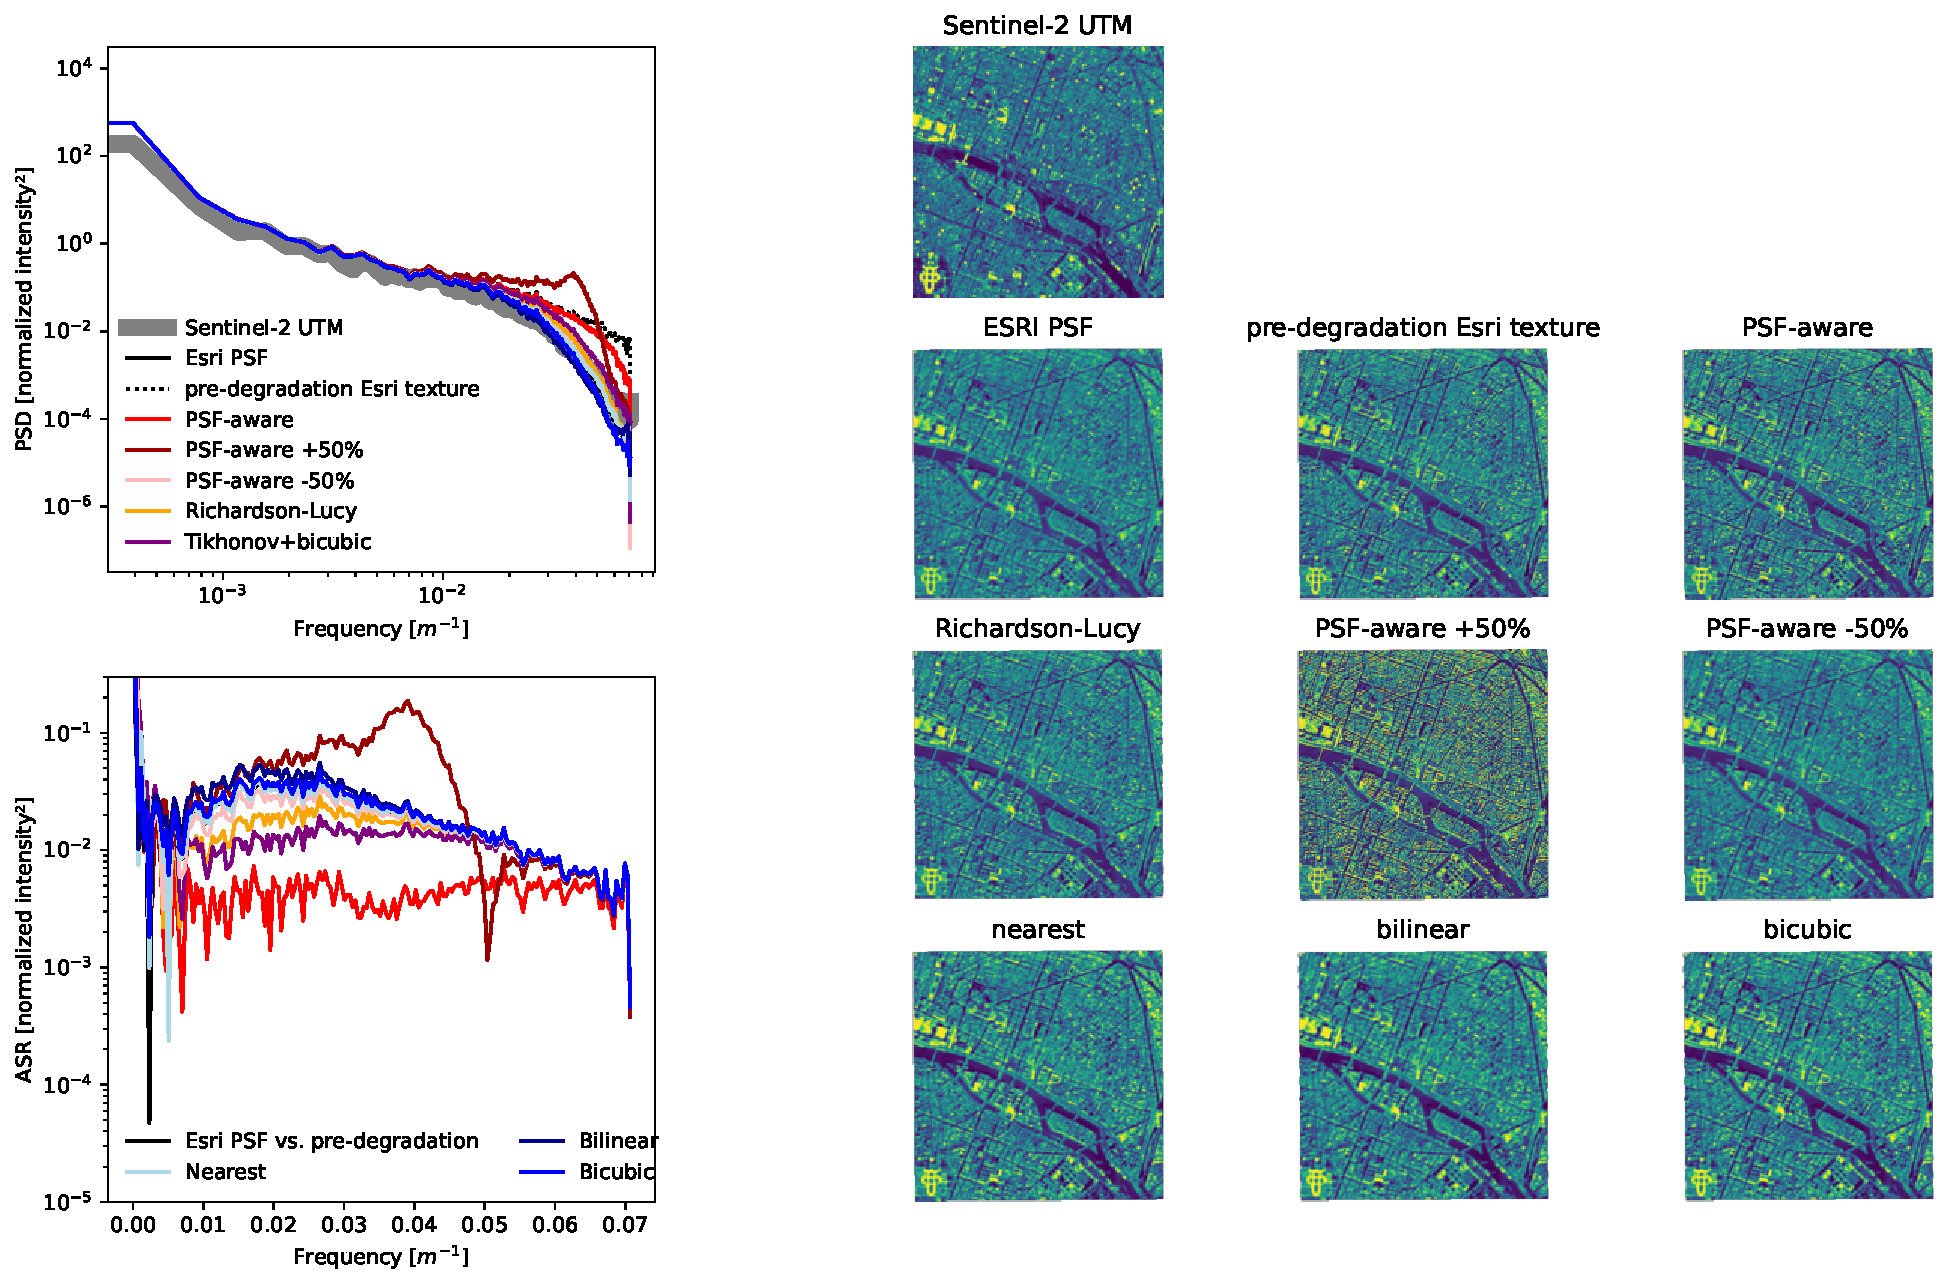
\includegraphics[width=0.98\linewidth]
    {figures/resample-test.pdf}
    \caption{Spatial and spectral diagnostics for the urban
    synthetic-detector experiment at \healpix level~20.
    \emph{Right:} reference and reconstructed fields rendered on
    the \utm grid. \emph{Top left:} isotropically averaged
    one-dimensional power spectra. \emph{Bottom left:} absolute
    spectral residuals relative to the no-\psf latent texture,
    $\left|P_{\mathrm{est}}(k)
    -P_{\mathrm{no\text{-}PSF}}(k)\right|$.
    The matched \psf-aware reconstruction is closest to the
    no-\psf reference over most of the resolved frequency range.
    Richardson--Lucy and a non-iterative Tikhonov baseline
    (Section~\ref{sec:rl_ablation}), both evaluated after the same
    bicubic-upsampled, cell-averaged \healpix regridding, give
    similar but consistently larger residuals. Overestimating
    the operator width by $50\%$ produces strong high-frequency
    amplification, whereas underestimating it primarily results
    in incomplete restoration.}
    \label{fig:synthetic_overview}
\end{figure*}

\begin{figure*}[t]
    \centering
    
\includegraphics[width=\textwidth]
    {figures/all-spectra.pdf}
    \caption{Power spectral density (PSD) and absolute spectral residuals (ASR) for the water, forest, and agriculture scenes. The matched \psf-aware reconstruction produces the smallest discrepancy across most of the resolved frequency band in all three scenes. The Richardson--Lucy solution tracks it closely but consistently remains slightly worse. The oversized \psf-aware $+50\%$ setup shows high-frequency amplification, whereas the undersized \psf-aware $-50\%$ setup stays under-corrected. These mismatch effects are less pronounced than in the urban scene, which exhibits more fine-scale, high-contrast detail.}
    \label{fig:synthetic_spectra_other}
\end{figure*}

Fig.~\ref{fig:synthetic_overview} shows the urban case. The geometric
baselines remain close to the blurred observation
and further attenuate intermediate and high frequencies. The
matched reconstruction instead shifts the spectrum toward the
latent no-\psf texture and gives the smallest absolute spectral
residual over most of the resolved band. It does not recover the
highest frequencies fully, where the observation model is weakly
constraining; the result is therefore a stable partial
deconvolution rather than complete inversion.

The mismatch spectra explain their asymmetric RMSE. The $+50\%$
operator compensates for excessive assumed attenuation and
amplifies weakly constrained high-frequency components, which a common
damping does not suppress. The $-50\%$ operator applies too little
correction and remains under-restored without the same strong
instability.

Richardson--Lucy and the non-iterative Tikhonov baseline follow the
matched spectrum closely but retain larger residuals after the same
cell-average \healpix regridding. The water, forest, and agriculture
panels of Fig.~\ref{fig:synthetic_spectra_other} reproduce the urban
ordering, with weaker mismatch effects.
Together, the four scenes link the image-domain improvement to
partial recovery of attenuated spatial variability rather than to
a uniform radiometric shift.

\section{Real Sentinel-2 Round-Trip Sanity Check}
\label{sec:roundtrip_results}

Table~\ref{tab:roundtrip_metrics} reports the
\utm--\healpix--\utm round-trip consistency between the original
Sentinel-2 observation $\mathbf{y}$ and the prediction
$\widehat{\mathbf{y}}=\mathbf{A}\widehat{\mathbf{x}}$ obtained
from the reconstructed \healpix field.

For all four scenes, the \psf-aware method yields RMSE between
$2.8\times10^{-6}$ and $1.0\times10^{-5}$ (SSIM
$\geq0.99999997$), against $8.1\times10^{-4}$ to
$1.2\times10^{-2}$ for the geometric baselines.

These results show that the inferred \healpix representation
retains the information required to reproduce the original
projected-grid observation with a residual two to three orders of
magnitude below the geometric baselines, under the assumed forward
model. The residual is not at floating-point precision because the
matched reconstruction uses the light damping $\lambda=10^{-3}$ of
Section~\ref{sec:exp_config} rather than an undamped solve; the
round trip is thus a consistency and practical reversibility test
under the operating configuration used elsewhere in this paper
(Section~\ref{sec:roundtrip_interpretation}).

\begin{table*}[t]
\centering
\caption{Sentinel-2 \utm--\healpix--\utm round-trip sanity check.
RMSE and SSIM compare the original projected-grid observation
$\mathbf{y}$ with the prediction
$\widehat{\mathbf{y}}=\mathbf{A}\widehat{\mathbf{x}}$ reconstructed
from the \healpix field. These metrics assess observation
consistency rather than recovery of an unknown unblurred scene.
Bold indicates the best result for each scene.}
\label{tab:roundtrip_metrics}
\setlength{\tabcolsep}{5pt}
\begin{tabular}{lrrrrrrrr}
\toprule
 & \multicolumn{2}{c}{PSF-aware} & \multicolumn{2}{c}{Nearest-neighbor} & \multicolumn{2}{c}{Bilinear} & \multicolumn{2}{c}{Bicubic} \\
\cmidrule(lr){2-3}\cmidrule(lr){4-5}\cmidrule(lr){6-7}\cmidrule(lr){8-9}
Scene & RMSE & SSIM & RMSE & SSIM & RMSE & SSIM & RMSE & SSIM \\
\midrule
Urban       & $\mathbf{1.01\!\times\!10^{-5}}$ & $\mathbf{0.99999998}$ & $5.54\!\times\!10^{-3}$ & $0.9974$ & $1.21\!\times\!10^{-2}$ & $0.9559$ & $1.20\!\times\!10^{-2}$ & $0.9602$ \\
Water       & $\mathbf{3.48\!\times\!10^{-6}}$ & $\mathbf{0.99999999}$ & $1.05\!\times\!10^{-3}$ & $0.9949$ & $4.27\!\times\!10^{-3}$ & $0.9860$ & $4.12\!\times\!10^{-3}$ & $0.9883$ \\
Forest      & $\mathbf{3.28\!\times\!10^{-6}}$ & $\mathbf{0.99999999}$ & $1.08\!\times\!10^{-3}$ & $0.9912$ & $4.15\!\times\!10^{-3}$ & $0.9663$ & $4.59\!\times\!10^{-3}$ & $0.9693$ \\
Agriculture & $\mathbf{2.84\!\times\!10^{-6}}$ & $\mathbf{0.99999999}$ & $8.08\!\times\!10^{-4}$ & $0.9958$ & $3.71\!\times\!10^{-3}$ & $0.9839$ & $4.69\!\times\!10^{-3}$ & $0.9822$ \\
\bottomrule
\end{tabular}
\end{table*}



\section{Measurement Noise and Geolocation Robustness}
\label{app:noise_geoloc}

\subsection{Noise Sensitivity Under the Matched \psf}
\label{sec:noise_matched}

We complement the deterministic experiment of
Section~\ref{sec:controlled_synthetic} with a repeated
$\mathbf y=\mathbf A\mathbf x+\mathbf n$ experiment in which
$\mathbf n$ is either white Gaussian noise or spatially correlated
Gaussian noise obtained by Gaussian smoothing with a width of
$1.5$ source pixels and subsequent variance renormalization. Five
nominal SNR levels, from 100 to 5, are used to generate the
perturbations, but the analysis is reported against the resulting
absolute input-noise standard deviation $\sigma_n$. This avoids
treating a fixed SNR as the same noise amplitude in scenes having
different radiometric variance.

We test $\lambda\in\{0,10^{-3},10^{-2},10^{-1},1\}$ on the four
scenes, using ten independent noise realizations per configuration.
The same realization is shared across the five damping values so
that their comparison is paired. To retain the bias introduced by
regularization, every noisy result is compared with the same clean,
undamped reference. We define the excess reconstruction error as

\begin{equation}
E_{\lambda}(\sigma_n)=
\sqrt{\max\!\left\{
\operatorname{RMSE}_{\mathrm{noise},\lambda}^{2}
-\operatorname{RMSE}_{\mathrm{clean},0}^{2},\,0
\right\}}.
\label{eq:noise_excess_error}
\end{equation}

Using the clean result at the corresponding $\lambda$ instead would
remove the regularization bias and make progressively stronger
damping appear artificially favourable. Equation~\eqref{eq:noise_excess_error}
instead exposes the complete trade-off relative to the noise-free,
undamped reconstruction.

\begin{figure}[t]
\centering

\includegraphics[width=\columnwidth]{noise_transfer_loglog.pdf}
\caption{Noise sensitivity across the four synthetic scenes, matched
\psf. The abscissa is the absolute standard deviation $\sigma_n$ of
the injected measurement noise, rather than the scene-dependent SNR.
The ordinate is the excess reconstruction error of
Eq.~\eqref{eq:noise_excess_error}, relative to the common clean
$\lambda=0$ result. Colours identify the damping value and marker
shapes identify the scene. Points show the mean over ten paired
noise realizations and error bars show one standard deviation
(often smaller than the marker). White and spatially correlated
noise are shown separately. Every solve, including $\lambda=0$, uses
a zero CG initial vector and at most 14 iterations.}
\label{fig:noise_transfer}
\end{figure}

Figure~\ref{fig:noise_transfer} shows that the appropriate damping
depends on the anticipated noise level. For white noise, the lowest
tested amplitudes favour little or no explicit damping, whereas the
preferred value shifts toward $\lambda=10^{-1}$ or $1$ as
$\sigma_n$ increases. Strong damping is therefore useful when
white-noise amplification dominates, but its non-zero error floor
becomes detrimental for cleaner data. The transition varies across
scenes, consistent with differences in their spatial spectra and in
the fraction of fine-scale structure that is only weakly constrained
on a $6.22$~m target grid from 10~m measurements.

For the correlated-noise model tested here, $\lambda=0$ gives the
lowest excess error across all four scenes and all five noise
levels. Increasing $\lambda$ then adds more bias than the amount of
correlated error it removes. This result is specific to the chosen
correlation scale and to the common zero-initialized, at-most-14-step
CG rule. In particular, it does not establish a unique undamped
solution and should not be generalized to arbitrary stopping rules
or noise covariances.

The ordinate in Fig.~\ref{fig:noise_transfer} should not be read as
an estimate of sensor noise alone. It combines propagation of the
injected perturbation with the response of weakly constrained
small-scale degrees of freedom and, for $\lambda>0$, the retained
regularization bias. This is precisely why an absolute noise scale
is more interpretable here than SNR alone. In principle, $\lambda$
could be selected from an expected noise amplitude and covariance,
the source-to-target resolution ratio, and local scene structure.
The present paper does not attempt such dynamic selection: the main
matched comparison retains the fixed $\lambda=10^{-3}$ configuration.
Developing and validating a noise-adaptive rule, for example through
a discrepancy principle, generalized cross-validation, or a
hierarchical noise model, is left to a dedicated study. This
experiment remains limited to one patch per scene type
(Section~\ref{sec:generalization}).

A multi-date extension of the controlled reduced-resolution protocol would
provide realistic sensor and atmospheric perturbations. It is left
for future work because it requires cloud-free repeat coverage and a
separate treatment of genuine surface change. Repeating only the
round trip would test self-consistency rather than reconstruction
quality.

\subsection{Interaction Between Noise and \psf Mismatch}
\label{sec:noise_psf_mismatch}

The sweep of Appendix~\ref{sec:noise_matched} uses only the matched
\psf configuration. We repeat it, at the same five SNR levels and
ten paired realizations, for the $\pm50\%$ mismatch configurations
of Section~\ref{sec:psf_mismatch}, each evaluated at its own
per-arm damping ($\lambda=0.01$ for matched and $-50\%$, $\lambda=0.1$
for $+50\%$). These values define a separate arm-specific robustness
comparison selected from the damping sweep; they are not the common
$\lambda=10^{-3}$ configuration of Table~\ref{tab:synthetic_metrics}.
This directly tests the \psf-mismatch configurations jointly with
measurement noise rather than only at the matched configuration.

\begin{figure}[t]
\centering

\includegraphics[width=\columnwidth]{noise_psf_mismatch_summary.pdf}
\caption{RMSE against the pre-degradation reference, under white and
spatially correlated noise, for the matched and $\pm50\%$
mismatched \psf configurations, each at its own per-arm damping.
Points are the mean over the four scenes at each SNR level.}
\label{fig:noise_psf_mismatch}
\end{figure}

Fig.~\ref{fig:noise_psf_mismatch} summarizes the resulting
behaviour across SNR levels, and
Table~\ref{tab:noise_psf_mismatch} reports the RMSE against the
pre-degradation reference under white noise for the two extreme tested
SNR levels. At the mild-noise end (SNR$=100$, close to the
noise-free case), the matched configuration remains the best in
every scene, consistent with Section~\ref{sec:synthetic_results}.
At the severe-noise end (SNR$=5$), this ranking reverses in all
four scenes: a mismatched configuration achieves a \emph{lower}
RMSE than the matched configuration. This is not evidence that
\psf mismatch is beneficial. Two confounded effects are at play:
underestimating the \psf width leaves the inversion
under-correcting the blur, which incidentally behaves like extra
implicit regularization against noise; and the $+50\%$ arm is
evaluated at a ten-times stronger explicit damping ($\lambda=0.1$
instead of $0.01$) specifically because that configuration is
otherwise the most ill-conditioned; this arm-specific choice is used
only for the robustness comparison and likewise suppresses noise at
the cost of bias. Both effects trade restoration accuracy for noise
robustness. Under the common $\lambda=10^{-3}$ comparison, both width
mismatches already degrade the noise-free reconstruction relative to
the matched configuration (Table~\ref{tab:synthetic_metrics}); the
present arm-specific damping adds a second, explicit bias--variance
trade-off. The practical implication is
that \psf-mismatch robustness and noise-damping robustness cannot
be tuned independently: a damping value chosen only from an assumed
noise level, or a \psf width chosen only from a clean-data accuracy
target, can silently interact in either direction.

\begin{table}[t]
\centering
\caption{RMSE against the pre-degradation reference, white noise, at the
two extreme tested SNR levels, for the matched and $\pm50\%$ \psf
configurations at their respective per-arm damping. Bold indicates
the lowest RMSE in each row.}
\label{tab:noise_psf_mismatch}
\begin{tabular}{llrrr}
\toprule
Scene & SNR & Matched & $-50\%$ & $+50\%$ \\
\midrule
Agriculture & 5   & 0.0694 & \textbf{0.0354} & 0.0360 \\
Agriculture & 100 & \textbf{0.0160} & 0.0225 & 0.0186 \\
Forest      & 5   & 0.0628 & 0.0407 & \textbf{0.0395} \\
Forest      & 100 & \textbf{0.0246} & 0.0333 & 0.0295 \\
Urban       & 5   & 0.0962 & 0.1014 & \textbf{0.0907} \\
Urban       & 100 & \textbf{0.0693} & 0.0977 & 0.0855 \\
Water       & 5   & 0.0620 & 0.0392 & \textbf{0.0375} \\
Water       & 100 & \textbf{0.0216} & 0.0314 & 0.0265 \\
\bottomrule
\end{tabular}
\end{table}

\subsection{Geolocation Sensitivity}
\label{sec:geoloc_sensitivity}

We also test sensitivity to source-sample geolocation error.
Independent Gaussian perturbations are applied to each source
sample's longitude and latitude before the observation operator is
built, at three levels expressed in native detector pixels
($0.1$, $0.2$, $0.4$~px, i.e.\ approximately $1$, $2$, and $4$~m at
the $10$~m Sentinel-2 B04 sampling used throughout), with ten
independent realizations per level and per scene, at the matched
\psf and $\lambda=0.01$. Because the operator's geometry itself
depends on the (perturbed) source positions, the operator is
rebuilt for every realization rather than reused. For each scene,
the ten realizations perturb the same base patch; they are not ten
independently sampled geographic scenes.

\begin{figure}[t]
\centering

\includegraphics[width=\columnwidth]{geolocation_sensitivity.pdf}
\caption{RMSE against the pre-degradation reference as a function of
geolocation jitter standard deviation, for the matched \psf
configuration ($\lambda=0.01$). Error bars show one standard
deviation over ten perturbations of one base patch per scene.}
\label{fig:geoloc_sensitivity}
\end{figure}

Fig.~\ref{fig:geoloc_sensitivity} shows the resulting RMSE as a
function of jitter amplitude, and
Table~\ref{tab:geoloc_sensitivity} reports the relative RMSE
increase over the exact-geolocation baseline. Degradation is
monotonic and substantial: at $0.1$~px ($\approx1$~m) RMSE already
increases by $14$--$27\%$, and at $0.4$~px ($\approx4$~m) it
increases by $172$--$283\%$, more than doubling or tripling the
reconstruction error in every scene. Unlike the noise sweep above,
no damping-based mitigation is tested here: the mismatch is purely
geometric, between the assumed and the true source-sample location,
and is not the kind of error that regularization against noise
suppresses. This confirms that sub-pixel geolocation accuracy is a
material requirement for the method, not a second-order concern,
and motivates the geolocation-correction terms outlined as future
work in Section~\ref{sec:generalization}.

\begin{table}[t]
\centering
\caption{RMSE increase relative to exact geolocation ($\sigma=0$),
matched \psf, $\lambda=0.01$, mean over ten realizations per level.}
\label{tab:geoloc_sensitivity}
\begin{tabular}{lrrr}
\toprule
Scene & $0.1$~px & $0.2$~px & $0.4$~px \\
\midrule
Agriculture & $+27\%$ & $+101\%$ & $+283\%$ \\
Forest      & $+15\%$ & $+61\%$  & $+184\%$ \\
Urban       & $+14\%$ & $+57\%$  & $+172\%$ \\
Water       & $+18\%$ & $+71\%$  & $+204\%$ \\
\bottomrule
\end{tabular}
\end{table}

\section{Throughput and Batch-Scaling Benchmark}
\label{app:throughput_scaling}

Section~\ref{sec:hpx_datacube_implications} times one patch at a time.
A dedicated notebook benchmark on the same NVIDIA L4 (22~GiB)
system as
Section~\ref{sec:hpx_datacube_implications} draws its patch pool
from the 40 archived real Sentinel-2 region patches of the Zenodo bundle
(falling back, when those are absent, to the Esri cache or to the
site-manifest geometries with deterministic synthetic textures;
construction cost depends on geometry only) and times
batch sizes from 1 to 2048
under three
regimes: one operator shared across a batch of repeated acquisitions
of the same footprint (independent per-item radiometric noise only);
the same footprint with the operator rebuilt every item, a naive
baseline isolating the benefit of reuse; and a batch of real,
distinct cached patches (operator necessarily rebuilt each time).
Each regime and batch size was run once, so the results characterize
the observed scaling sweep rather than repeat-to-repeat uncertainty;
no confidence interval across independent benchmark runs can be
reported.

\begin{figure}[t]
\centering

\includegraphics[width=\columnwidth]{throughput_scaling_curve.pdf}
\caption{Observed wall time per patch in one batch-scaling sweep, for
the three regimes described in the text.}
\label{fig:throughput_scaling}
\end{figure}

Figure~\ref{fig:throughput_scaling} shows the observed scaling curve.
Over the 8190 timed builds, per-item operator construction
has a median of $0.766$~s (interquartile range $0.740$--$0.795$~s).
This is deliberately not comparable with the per-patch construction
figure of Section~\ref{sec:hpx_datacube_implications}: the benchmark
runs in a separate process on a different patch pool (the archived
Sentinel-2 regions, whose per-store curvilinear coordinate grids
differ from the synthetic-geometry patches timed there, and
construction cost depends on geometry), so only comparisons within
this sweep are meaningful. Within it,
the per-batch-size medians span $0.37$--$1.10$~s with the
smallest batches slowest, and 436 builds exceed 1~s (the slowest
reaching $4.7$~s) --- consistent with warm-up and with contention
on a shared accelerator, so the per-batch figures should be read
accordingly. The solve is highly reproducible at a
median of $0.073$~s regardless of batch size.
Sharing one operator across a batch amortizes construction away:
at batch size 2048, the shared-operator regime reaches
$0.075$~s/patch ($47{,}709$~patches/h), against $0.861$~s/patch
($4{,}182$/h) for the same footprint rebuilt every time and
$0.868$~s/patch ($4{,}148$/h) for 2048 draws over the 40-patch
Sentinel-2 pool (with replacement beyond 40; all 40 patches were
drawn at least once).
This single sweep gives an observed $11.4\times$--$11.5\times$ speedup from
operator reuse, quantifying the argument of
Section~\ref{sec:hpx_datacube_implications}: repeated acquisitions of
the same footprint benefit substantially from reuse, while batches of
distinct geographic patches do not.

\section{Exact Conservation of Area-Integrated Quantities}
\label{app:conservative}

The main text addresses spatial fidelity under an assumed sensor
response. Some applications impose a different requirement:
preserving an area-integrated quantity exactly when a field is
transferred between grids. This is essential for fluxes used in
budget calculations, boundary conditions, and coupling terms in
Earth-system models.

This appendix presents two optional conservation paths implemented
in \texttt{healpix-resample}. The first adds a global linear
constraint to the smooth \psf-aware reconstruction. The second is
a purely algebraic hard-binning operator that conserves the
discrete area-weighted source sum by construction. Neither method
is used in the Sentinel-2 experiments of the main paper. Their
purpose is to support applications for which integrated
conservation, rather than spatial restoration alone, is required.


\subsection{Relation to Conservative Remapping Tools}
\label{sec:related_conservative}

Conservative remapping is well established in climate and
Earth-system modeling. SCRIP, ESMF, xESMF, and TempestRemap
construct conservative weights from intersections between
finite-area source and target cells
\cite{jones1999scrip,hill2004esmf,zhuang2020xesmf,
ullrich2015tempestremap}.

The hard-binning method introduced below addresses the same
conservation objective but uses a different construction: source
samples are treated as area-weighted points and assigned to a
single \healpix cell. It therefore conserves the resulting
discrete weighted sum exactly, but it is not a polygon-overlap
remapper. The constrained \psf-aware method instead preserves the
smooth kernel-based reconstruction while imposing a prescribed
global integral.


\subsection{Optional Flux-Conservation Constraint}
\label{sec:conservative_constraint}

The correction defined by Eq.~\eqref{eq:correction_system}
minimizes an observation-space residual but does not guarantee
preservation of an area-integrated source quantity. Let $a_i$ be
the area, or more generally the extensive weight, associated with
source sample $i$.

For a complete global remapping, or whenever the total area of the
retained target support equals that of the source support,
conservation can be expressed as equality of the source and target
area-weighted means. Because the retained \healpix cells are
equal-area, this becomes

\begin{equation}
\frac{1}{M}\sum_{j=1}^{M}\widehat x_j
=
\frac{\sum_{i=1}^{N}y_i a_i}
     {\sum_{i=1}^{N}a_i}.
\label{eq:flux_constraint}
\end{equation}

The same source weights $a_i$ are used in the construction of
$\mathbf B$ and in Eq.~\eqref{eq:flux_constraint}, ensuring a
consistent area convention.

Let $\mathbf c=\mathbf 1_M$ and define

\begin{equation}
g
=
F-\mathbf c^{\mathsf T}\mathbf x_{\mathrm{ref}},
\end{equation}

where $F$ is the right-hand side of
Eq.~\eqref{eq:flux_constraint} multiplied by $M$. The constrained
correction minimizes the weighted objective of
Eq.~\eqref{eq:weighted_variational} subject to

\begin{equation}
\mathbf c^{\mathsf T}\boldsymbol\delta_{\mathrm{cons}}=g.
\end{equation}

Introducing a Lagrange multiplier $\nu$ gives

\begin{equation}
\mathbf H\boldsymbol\delta_{\mathrm{cons}}
=
\mathbf B\mathbf r_{\mathrm{ref}}
+
\nu\,\mathbf D_x^{-1}\mathbf c,
\label{eq:constrained_system}
\end{equation}

with

\begin{equation}
\mathbf H=\mathbf B\mathbf A+\lambda\mathbf I.
\end{equation}

By linearity,

\begin{equation}
\boldsymbol\delta_{\mathrm{cons}}
=
\boldsymbol\delta+\nu\mathbf w,
\qquad
\mathbf H\mathbf w=\mathbf D_x^{-1}\mathbf c,
\end{equation}

where $\boldsymbol\delta$ is the unconstrained correction. The
multiplier is then

\begin{equation}
\nu
=
\frac{
g-\mathbf c^{\mathsf T}\boldsymbol\delta
}{
\mathbf c^{\mathsf T}\mathbf w
}.
\label{eq:conservative_multiplier}
\end{equation}

The right-hand side of the auxiliary system is
$\mathbf D_x^{-1}\mathbf c$, rather than $\mathbf c$, because the
minimum-distortion correction is defined in the
$\mathbf D_x$-weighted metric. Computing $\mathbf w$ requires one
additional matrix-free conjugate-gradient solve with the same
operator and weighted inner product as the unconstrained
correction. The asymptotic cost remains
$\mathcal O(n_{\mathrm{it}}qN)$, with approximately twice the
iteration budget.

Once $\boldsymbol\delta$ and $\mathbf w$ have been computed,
Eq.~\eqref{eq:conservative_multiplier} imposes the scalar
constraint algebraically. The remaining conservation error is
therefore governed primarily by floating-point evaluation of the
global sums and correction. The conjugate-gradient accuracy
instead controls how closely $\mathbf w$ approximates the
minimum-distortion correction direction.

\subsection{Hard-Binning Conservative Resampling}
\label{sec:hard_binning}

When a smooth reconstructed field is not required, exact
conservation can be obtained without a spatial kernel or an
iterative solve. The
\texttt{ConservativeResampler} assigns each source sample to one
\healpix cell and conserves the resulting discrete weighted sum.

Let $\mathcal S_k$ be the set of source samples whose locations
fall inside target cell $k$. The sets $\{\mathcal S_k\}$ form a
disjoint partition of the retained source samples. The extensive
quantity assigned to cell $k$ is

\begin{equation}
h_k
=
\sum_{i\in\mathcal S_k}v_i a_i,
\label{eq:hardbin_forward}
\end{equation}

and a coverage-weighted mean can be mapped back to the contributing
source samples as

\begin{equation}
\widehat v_i
=
\frac{h_k}{A_k},
\qquad
A_k
=
\sum_{i\in\mathcal S_k}a_i,
\qquad
i\in\mathcal S_k.
\label{eq:hardbin_inverse}
\end{equation}

Conservation follows directly from the partition:

\begin{equation}
\sum_k h_k
=
\sum_k\sum_{i\in\mathcal S_k}v_i a_i
=
\sum_{i=1}^{N}v_i a_i.
\label{eq:hardbin_identity}
\end{equation}

This identity holds up to floating-point summation error and is
independent of the source-grid regularity or target \healpix
resolution.

The quantity $h_k$ is an extensive cell total. The normalization
$A_k$ in Eq.~\eqref{eq:hardbin_inverse} is the total source weight
assigned to cell $k$, not necessarily the geometric area of the
complete \healpix cell. Consequently,
Eq.~\eqref{eq:hardbin_inverse} defines a source-coverage-weighted
density and ensures a self-consistent back projection; it should
not be interpreted as a polygon-overlap estimate of the complete
target-cell mean.

Hard binning is exact and inexpensive but does not model a spatial
response and produces a piecewise-constant representation. The
constrained \psf-aware method instead retains a smooth,
kernel-based reconstruction at the cost of an additional iterative
solve. The appropriate choice therefore depends on whether the
downstream application prioritizes a spatial-response model,
discrete conservation, or both.

\subsection{ERA5 Experimental Setup}
\label{sec:era5_experiment}

The conservation methods were evaluated using ERA5 surface
sensible heat flux (\texttt{sshf}), for which the global
area-integrated total is physically meaningful. Data were obtained
from the ECMWF \texttt{reanalysis-era5-complete} archive
(\texttt{stream=enda}) for the ten ensemble members
\texttt{number=0--9}, at forecast steps 3 and 6~h, on the native
N256 reduced Gaussian grid containing 348{,}528 points.

Because \texttt{sshf} is accumulated, the mean flux over the
3--6~h interval was obtained as

\begin{equation}
\mathrm{flux}
=
\frac{
\mathrm{sshf}(6\,\mathrm h)-\mathrm{sshf}(3\,\mathrm h)
}{
3\times3600\,\mathrm s
}.
\label{eq:deaccum}
\end{equation}

The resulting values span approximately
$[-350,310]\,\mathrm{W\,m^{-2}}$ across the ensemble.

Per-sample area weights $a_i$ were constructed from midpoint
latitude boundaries and the longitude spacing of each reduced
Gaussian-grid ring. By construction, their sum reproduces the
sphere area $4\pi R^2$ to floating-point precision. These weights
are required because the source points are not exactly equal-area:
the largest associated area is approximately $3.6$ times the
smallest.

Both methods target a nested level-6 \healpix grid
($N_{\mathrm{side}}=64$, $K=49{,}152$ cells). Hard binning uses
only the source values, coordinates, and area weights. The
constrained kernel-based reconstruction uses nine target
neighbours per source sample, a Gaussian scale tied to the
level-6 pixel size, $\lambda=10^{-3}$, at most 200
conjugate-gradient iterations, and a relative residual tolerance
of $10^{-8}$. The conservation constraint is enabled through
\texttt{conservative=True} and requires the additional solve
described above.

For ensemble member $b$, the conservation metric is

\begin{equation}
\varepsilon_b
=
\frac{
\left|\widehat F_b-F_b\right|
}{
\left|F_b\right|
},
\qquad
F_b
=
\sum_{i=1}^{N}\mathrm{flux}_{b,i}a_i,
\label{eq:conservation_error}
\end{equation}

where $\widehat F_b$ is the total recovered from the remapped
representation. For hard binning,
$\widehat F_b=\sum_k h_{b,k}$. For the constrained reconstruction,
it is obtained from the target mean and the total source area,
consistently with Eq.~\eqref{eq:flux_constraint}.


\subsection{Results: Flux Conservation on ERA5 Data}
\label{sec:era5_results}

\begin{figure}[t!]
\centering
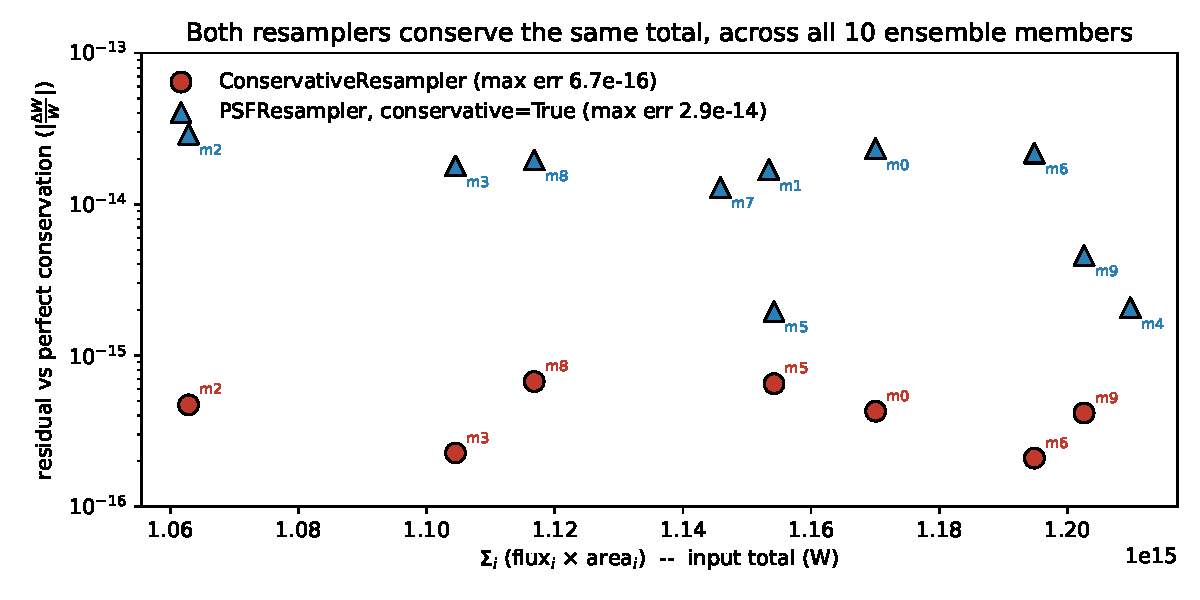
\includegraphics[width=\columnwidth]{conservative_proof.pdf}
\caption{Relative error in the global area-integrated ERA5
surface sensible heat flux for all ten ensemble members. Results
are shown for the hard-binning
\texttt{ConservativeResampler} and the constrained kernel-based
operator at \healpix level~6. Maximum relative errors are
$3.9\times10^{-16}$ and $2.9\times10^{-14}$, respectively.}
\label{fig:conservative_proof}
\end{figure}

Both methods preserve the global area-integrated total for every
ensemble member. The maximum relative error is
$3.9\times10^{-16}$ for hard binning and
$2.9\times10^{-14}$ for the constrained reconstruction
(Fig.~\ref{fig:conservative_proof}). These errors are negligible
relative to any physical variability in the tested fields.

For hard binning, the result follows from the exact regrouping of
the finite weighted source sum in
Eq.~\eqref{eq:hardbin_identity}; the observed residual is
consistent with double-precision summation. For the constrained
operator, the scalar equality is imposed by
Eq.~\eqref{eq:conservative_multiplier}, and the residual reflects
finite-precision evaluation of the global sums and corrected
field. The conjugate-gradient tolerance primarily affects the
accuracy of the minimum-distortion correction, rather than the
algebraic satisfaction of the scalar constraint.

The experiment therefore verifies that both implementations
preserve the requested global integral, while producing different
spatial representations. Hard binning provides an unconditional
discrete conservation identity but no spatial-response model. The
constrained operator combines conservation with a smooth
kernel-based reconstruction. Conservation of the scalar total does
not, by itself, assess spatial fidelity or prove optimality of the
reconstructed field; these properties must be evaluated
separately.

The two methods should consequently be regarded as complementary
options rather than competing estimators. Hard binning is suited
to applications requiring a simple and exactly conserved
discrete transfer, whereas the constrained formulation is useful
when conservation must be combined with the observation model of
the main method.



\balance
\section*{Data and Reproducibility}
The supplementary figures and tables are generated by the public notebooks in
\url{https://github.com/GRID4EARTH/healpix-resample}
\cite{healpix_resample_repo}, using the frozen input archive under DOI
\url{https://doi.org/10.5281/zenodo.22210945}
\cite{healpix_resample_paper_data}.

Cross-references to sections and equations of the main paper use label
numbers frozen at submission (\texttt{main-refs.tex}); regenerate that file
if the main paper is renumbered. Citations below are
numbered locally to keep this supplement self-contained.

\bibliographystyle{IEEEtran}
\bibliography{references}
\end{document}
